%!TEX root = article.tex

\section{Appendix}
\label{s:Appendix}

Additional material such as extra figures.

\subsection{Additional Material for the Green's Function Method}
%Put all the extra plots etc. from Green's Function Code here.

\subsubsection{General Structure of the Used Code}
\label{GreensCode}
%Explain everything about the code

In this section, an insight to the code provided by Secomb et al. \cite{Secomb2004} will be given. Especially some explanations about what data this code uses and what data it computes will be given. 
The main goal is to understand what the results are, how correct their accuracy is. For this, a general explanation of the structure and organization of the code and the methods behind the computations will given.

\subsubsection*{Inputs}
\label{Inputs}
%What data this code actually needs and what this data is

What are the inputs for this code ? Where do they come from ?
\\
\\The Green's Function Method takes .dat-files as inputs, which basically contain the network files.
\\
The input data in form of .dat-files is basically build out of four files:
\\- SoluteParams.dat: This file contains all the information about the solutes we are looking at. This information can be things like tissue solubility, Michaelis constant of consumption, etc.
\\- Network.dat: This file contains all the information about the network we are looking at. This information is basically in form of an array. This array defines for each segment the type, the start point, the end point, the diameter (in microns), the relativ flow (?) and the hematocrit (?).
\\- IntravascRes.dat: This file contains all the information about a diameter (which one?) and the intravascular resistance to radial oxygen transport K for each diameter/vessel.
\\- ContourParams.dat: This file contains all the information necessary to create the contour-plots. This means that we create a plot, where the oxygen concentration can be visualized on a 2-dimensional slice. (not sure how plot is created from this data?)
\\
\\The part of the code where the read-in of the network data and the sources (not sure about this) through the input files is being done is the input.cpp code.
\\
\\The analyzenet.cpp-part of the code analyzes the input-files...

\subsubsection*{Outputs}
\label{Outputs}
%What this code actually produces

What are the outputs for this code ? How are they produced ? Where do they come from ?
\\
\\The Green's Function Method gives .dat-files and images (contour.ps-files) as outputs, which basically contain the results that will be discussed later in the next chapters.
\\
\\The contour.ps-files are produced by the contour.cpp-part of the code, which basically generates and writes the data for the contour-plots. This data is a plot of the vessel from bottom to top according to the z-coordinate. One could see this plot as a 2D picture of a 3D network when looking from the bottom. A new pages is generated for each solute, and the computed solute concentration for each area is shown in colors.
\\
\\picturenetwork.cpp: picturenetwork.cpp - project network on z = 0 plane.
Uses parameters from CountourParams.dat
Labels nodes with nodvar and segments with segvar (must be float).
Generates a postscript file.
\\
The general outputs of the code can be classified into two categories:
\\- The first category is in the form of PostScript-files that can be visualized similar to pictures.
\\- The second category is in the form Text-files, containing the computed data.
\\

\subsubsection*{Organization of the Code}
%Briefly talk about each part of the code and explain how it all works together
%Might keep this part more general and mention each of the parts of the code like a puzzle in the Appendix

The code provided by Secomb et al. \cite{Secomb2004} consists of a few .cpp-files, so that tasks like input read-ins, calculations and output-file generations are separated. Each file has a specific role, which will be explained in detail in this section. As one can think, the most important part of this code is the implementation of the Green's Function Method and its application to the given data.
\\
%Solver bicgstab
\\The bicgstab.cpp-part of the code is the implementation of a solver based on the Parameter-free iterative linear solver by R. Weiss \cite{weiss1996parameter}.
\\
%blood
\\The blood.cpp-part of the code is quite interesting, as it basically does an important part of the calculation to obtain the oxygen concentration and distribution in the vessels and the tissue. In this part of the code
\\
%contr-lines
\\The contr-lines.cpp-part of the code generates the contour lines for these plots, whereas the contr-shade.cpp-part of the code generates the colors and the color bar on the side of the generated picture/plot.
\\
%convect
\\The convect.cpp-part of the code does the convective (flow) part of the calculation.
\\
%eval
\\The eval.cpp-part of the code does the evaluation of the solute field depending on the source strengths provided.
\\
%numerical methods (gaussj and ludcmp)
\\There are some numerical methods and mathematical calculations behind the simulation, as for example the Gauss-Jordan elimination or the Lower-Upper decomposition, which is implemented in the gaussj.cpp-part and the ludcmp.cpp-part of the code.
\\
%greens
\\The main implementation of the Green's Function Method is in the greens.cpp-part of the code, where Green's Function approach for multiple reacting species is implemented. (Talk more about this, heart of the code)
\\
%histogram
\\Histograms of solute levels are evaluated in the histogram.cpp-part of the code.
\\
%initgreens
\\Initial tissue source strengths (given uniform solute field) are computed in the initgreens.cpp-part of the code.
\\
%main
\\The code main.cpp calls the greens.cpp-code.
\\
%nrutil (.cpp and .hh)
\\The code nrutil.cpp/nrutil.hh is declaring variables and is allocating them.
\\
%outboun (method?)
\\Outboun.cpp: method = 1: finds the smallest convex region inside the cuboid
which excludes tissue node points that have a distance to the nearest
vessel greater than a value specified by the user (lb).  Any point
outside a region between two planes containing the required points is
excluded.  This is repeated for multiple plane orientations, determined by am.
\\
\\method = 2: finds all tissue points within a distance lb of the vessels, but
does not make a convex region.  Fills in 'holes' in interior, whether 2D or 3D.
\\
\\Output:	nnt, total tissue node points inside the region.
nbou > 1 if inside region, value gives tissue point index
\\
%putrank
\\putrank.cpp: generate nodes in order of flow direction
\\
%readsources
\\readsources.cpp: read source strengths from file (from TissueSources.out and VesselSources.out)
\\
%setuparrays 0, 1, 2
\\setuparrays0.cpp: set up arrays with fixed dimensions (for Green's)
\\
\\setuparrays1.cpp: set up arrays with dimensions of nnod and nseg (for Green's)
\\
\\setuparrays2.cpp: set up arrays with dimensions of nnv and nnt (for Green's)
\\
%testconvect
\\testconvect.cpp: testing if convect is giving correct results for alpha (?) matrix. Comparing matrix values with values obtained by numerical differentiation.
\\
%tissrate
\\tissrate.cpp: computing tissue uptake rates of solutes as a function of solute levels (concentration)
\\
\\Everyone of these code-parts is using the nrutil.hh code, why ?

\subsubsection{Some More Green's Results}

Figure \ref{fig:Contour_Cardiac}  is the result of a Green's Method blood flow simulation computed on a Cardiac network. The Solute Concentration in the network is visualized.\\
\begin{figure}[h]
\centering
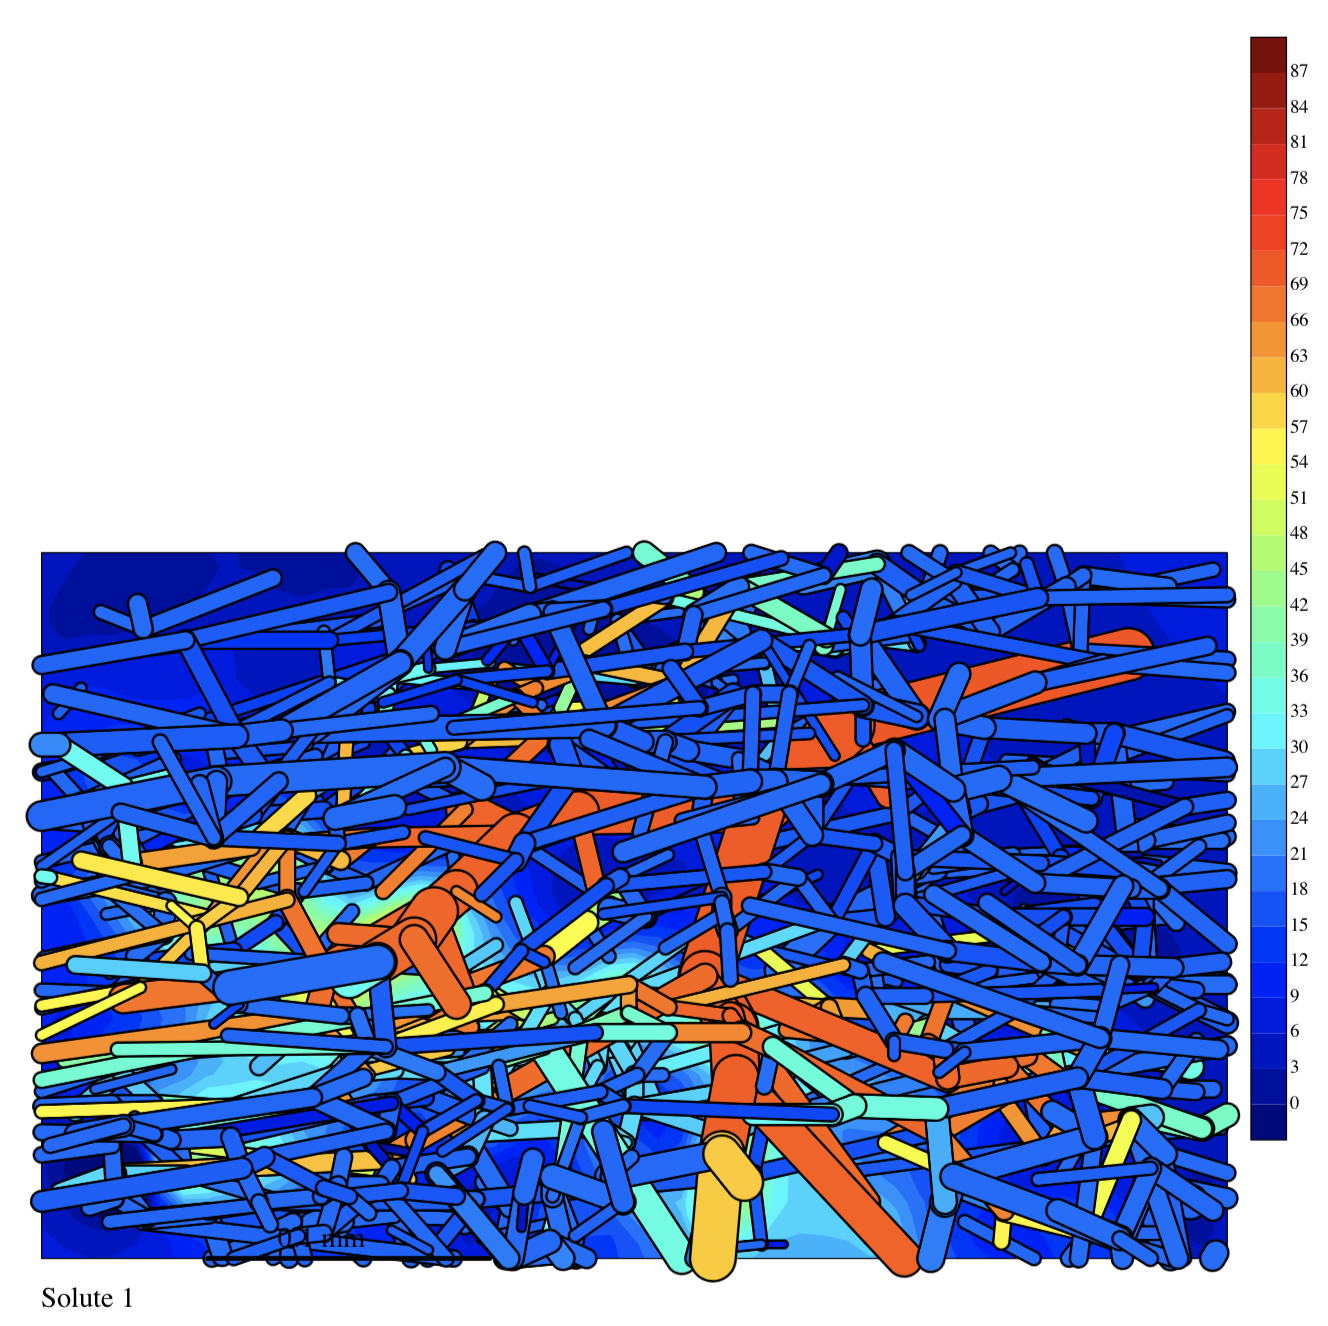
\includegraphics[width=170mm]{Contour_Cardiac}
\caption{Green's Contour Output for Cardiac Network}
\label{fig:Contour_Cardiac}
\end{figure}
\\
\begin{figure}[h]
\centering
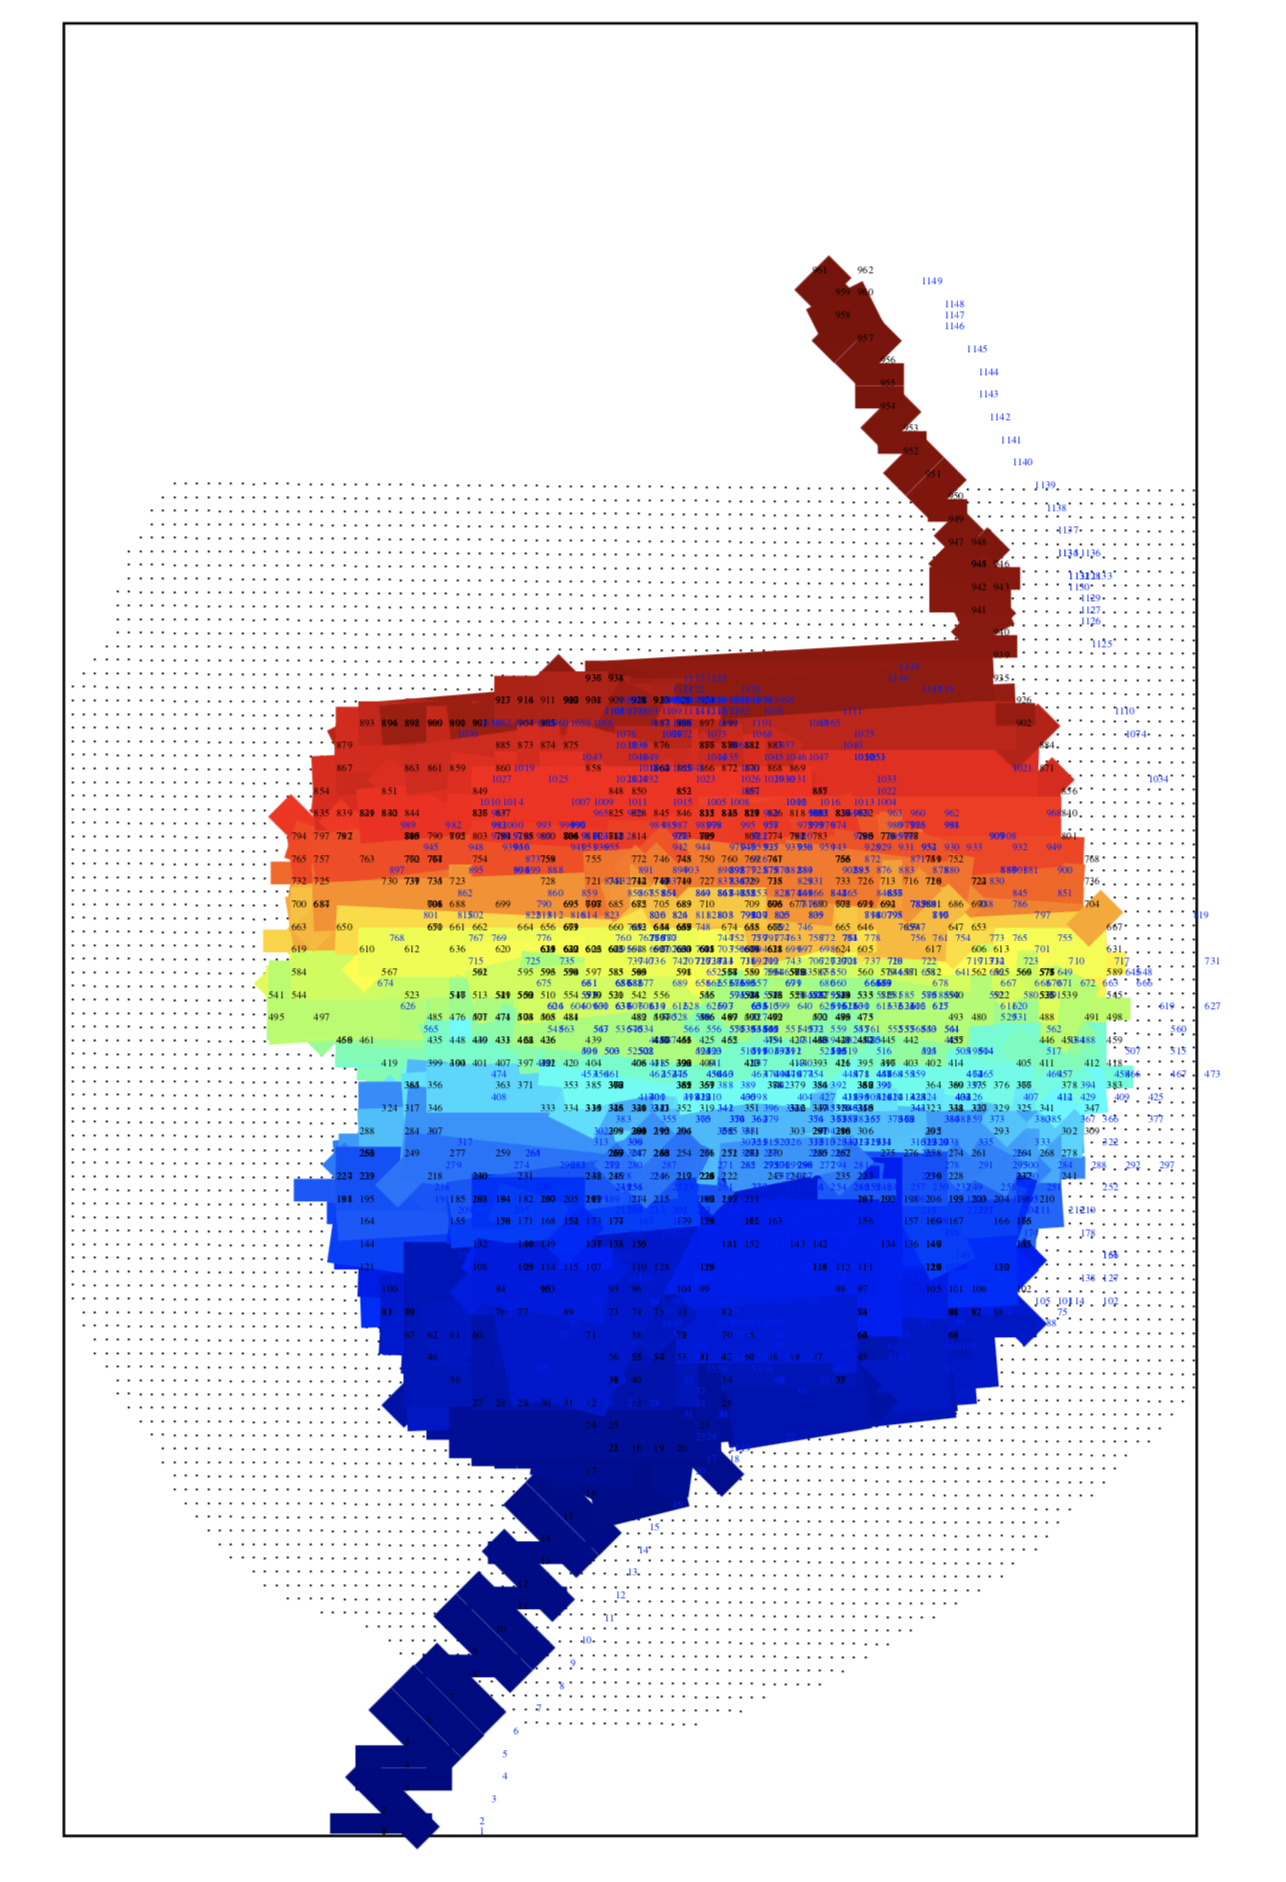
\includegraphics[width=100mm]{NetNodesSegs_Glom}
\caption{\footnotesize Green's Net Nodes Output for a Glomerulus Network}
\label{fig:NetNodesSegs_Glom}
\end{figure}

\subsection{Additional Material for DuMuX}
%Put all the extra images from ParaView here.

%\newpage
%\subsubsection{Some Glomerulus Network Simulation Results}
%Just to have some more figures

%\begin{figure}[h]
%\centering
%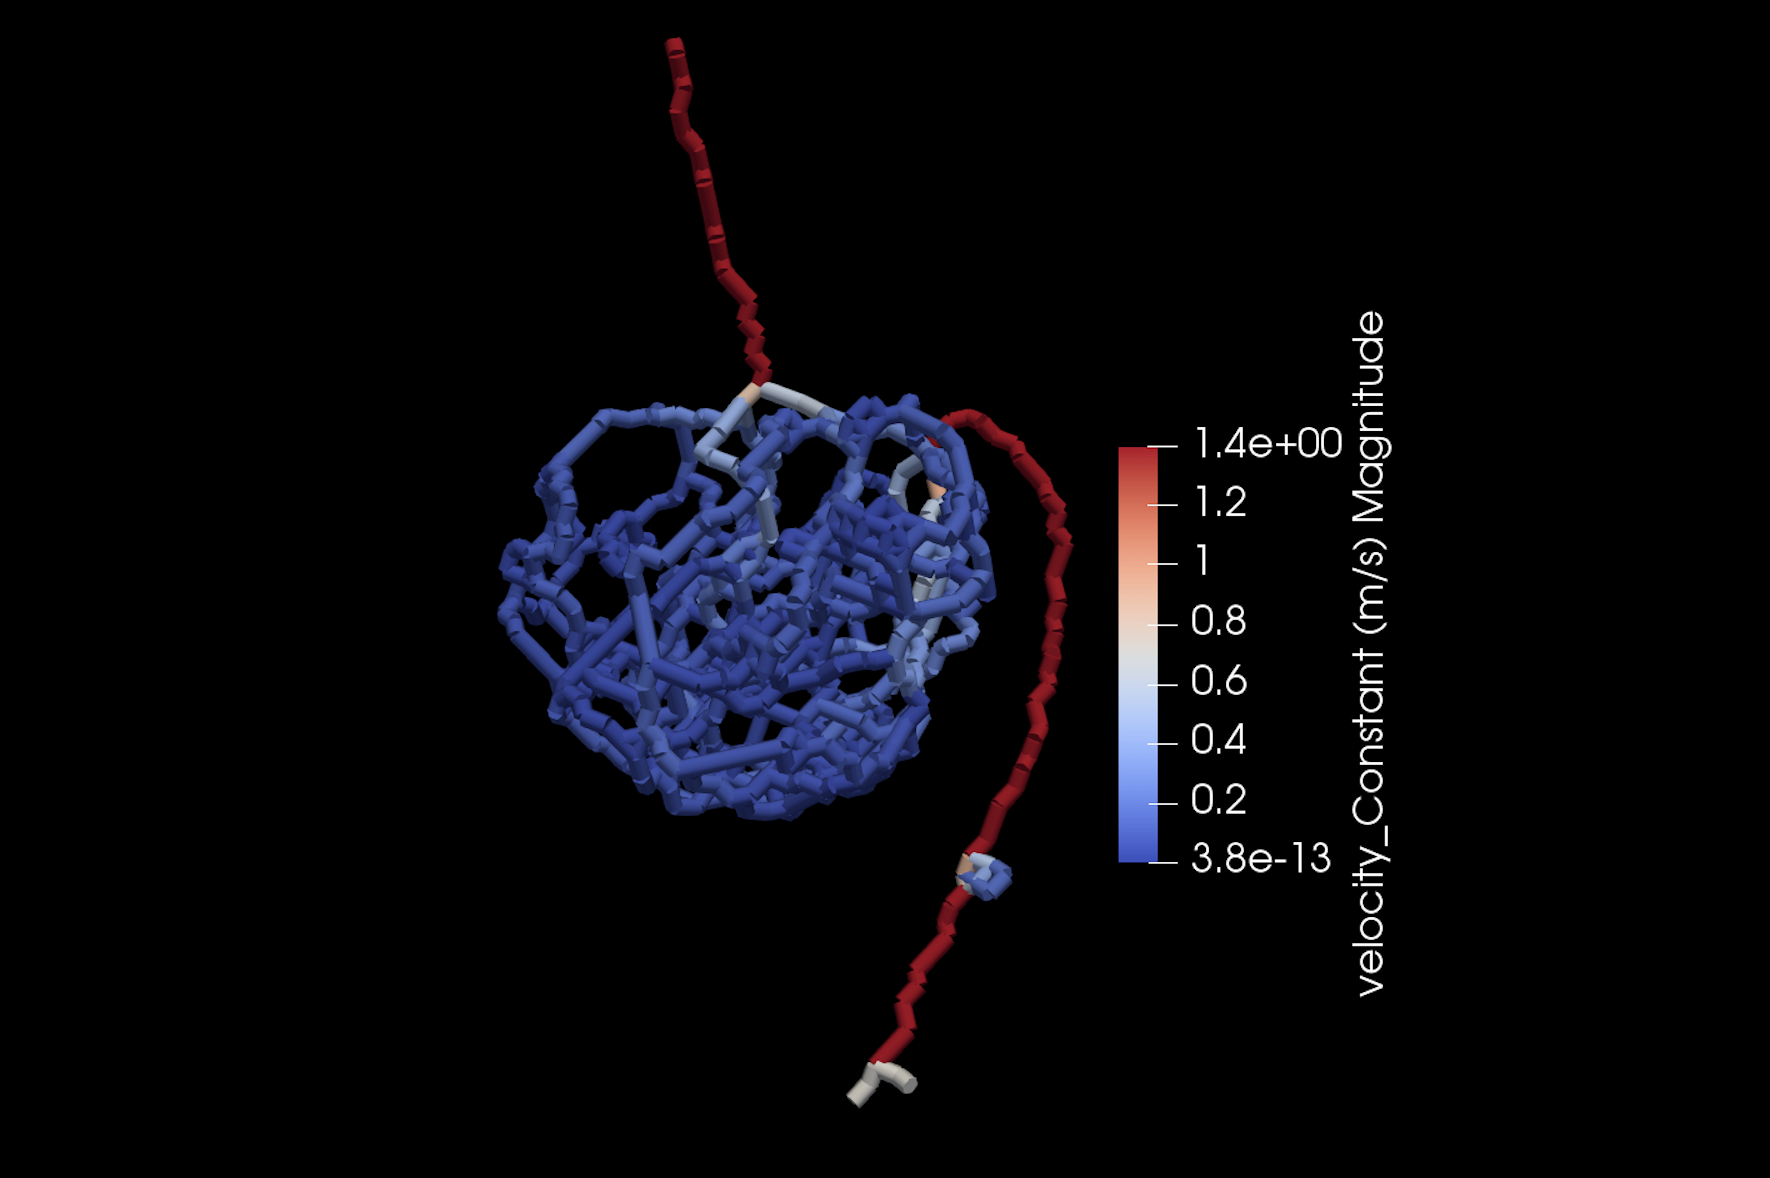
\includegraphics[width=162mm]{glom_velocity}
%\caption{Velocity Field in a Glomerulus}
%\label{fig:glom_velocity}
%\end{figure}
%The figure \ref{fig:glom_velocity} is the result of a DuMuX 1p-1p blood flow simulation computed on a glomerulus network. The velocity field of the flow is visualized.\\

%\begin{figure}[h]
%\centering
%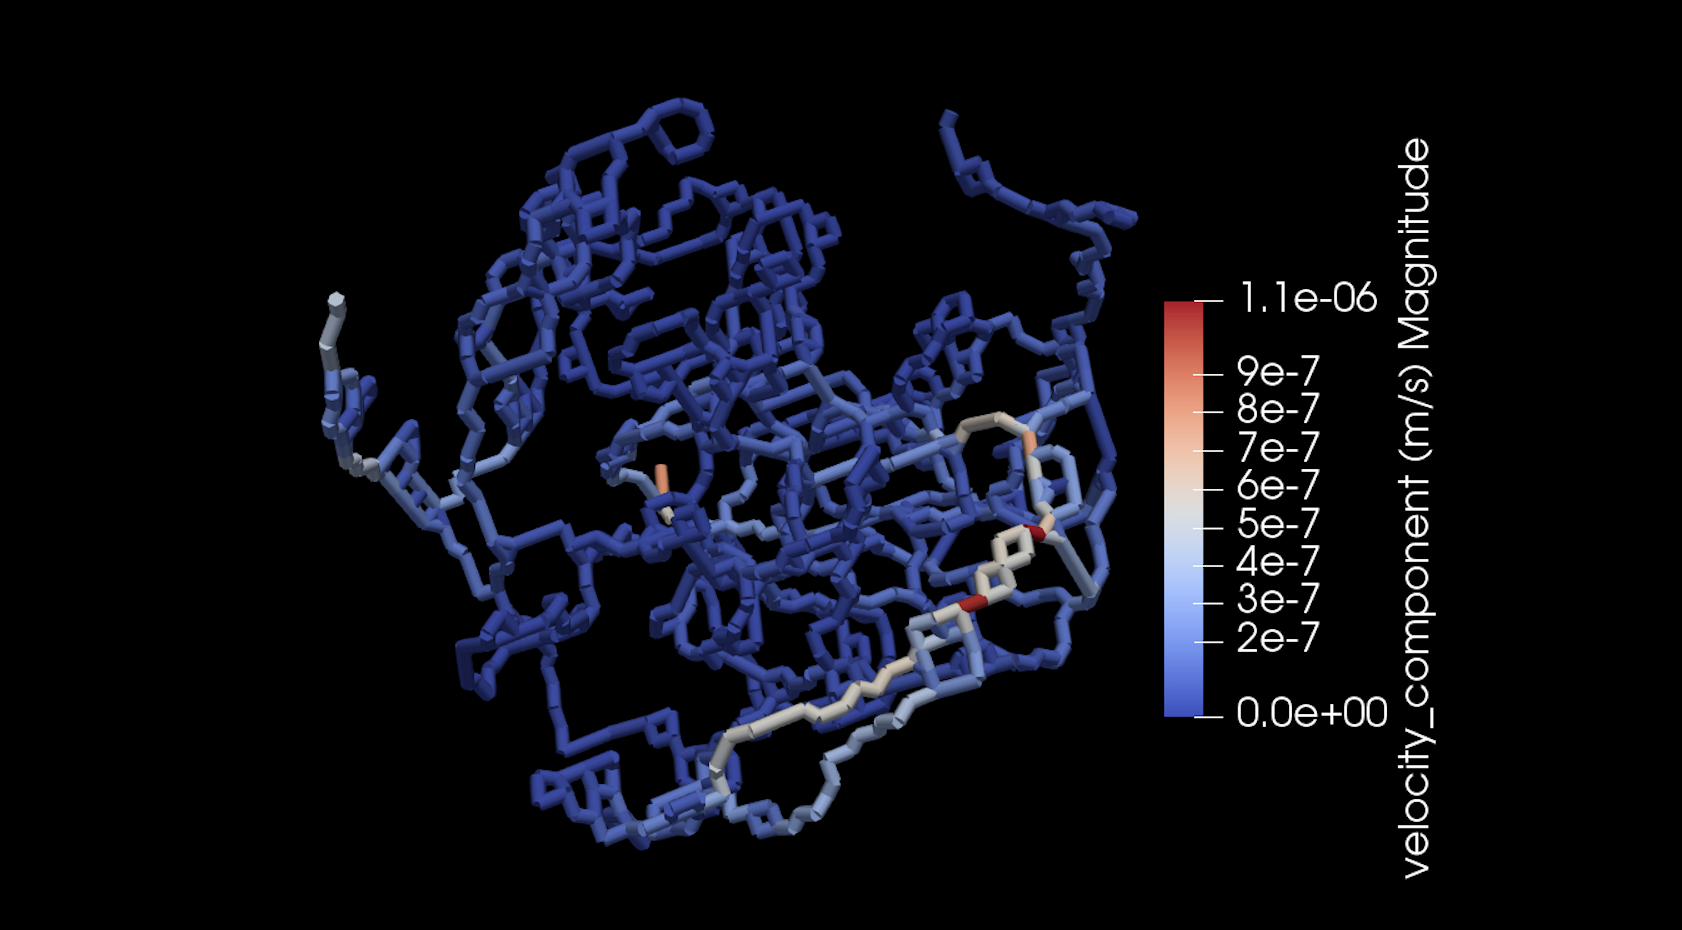
\includegraphics[width=162mm]{glom2_velocity}
%\caption{Velocity Field in a Glomerulus}
%\label{fig:glom2_velocity}
%\end{figure}
%The figure \ref{fig:glom2_velocity} is the result of a DuMuX 1p-1p blood flow simulation computed on a glomerulus network. The velocity field of the flow is visualized.\\

\subsubsection*{Some Tracer Simulations}
\label{Tracer}

This simulation is a simple diffusion of Groundwater in a porous rock. The velocity field of the solute is assumed to be constant.
\begin{figure}[h]
\centering
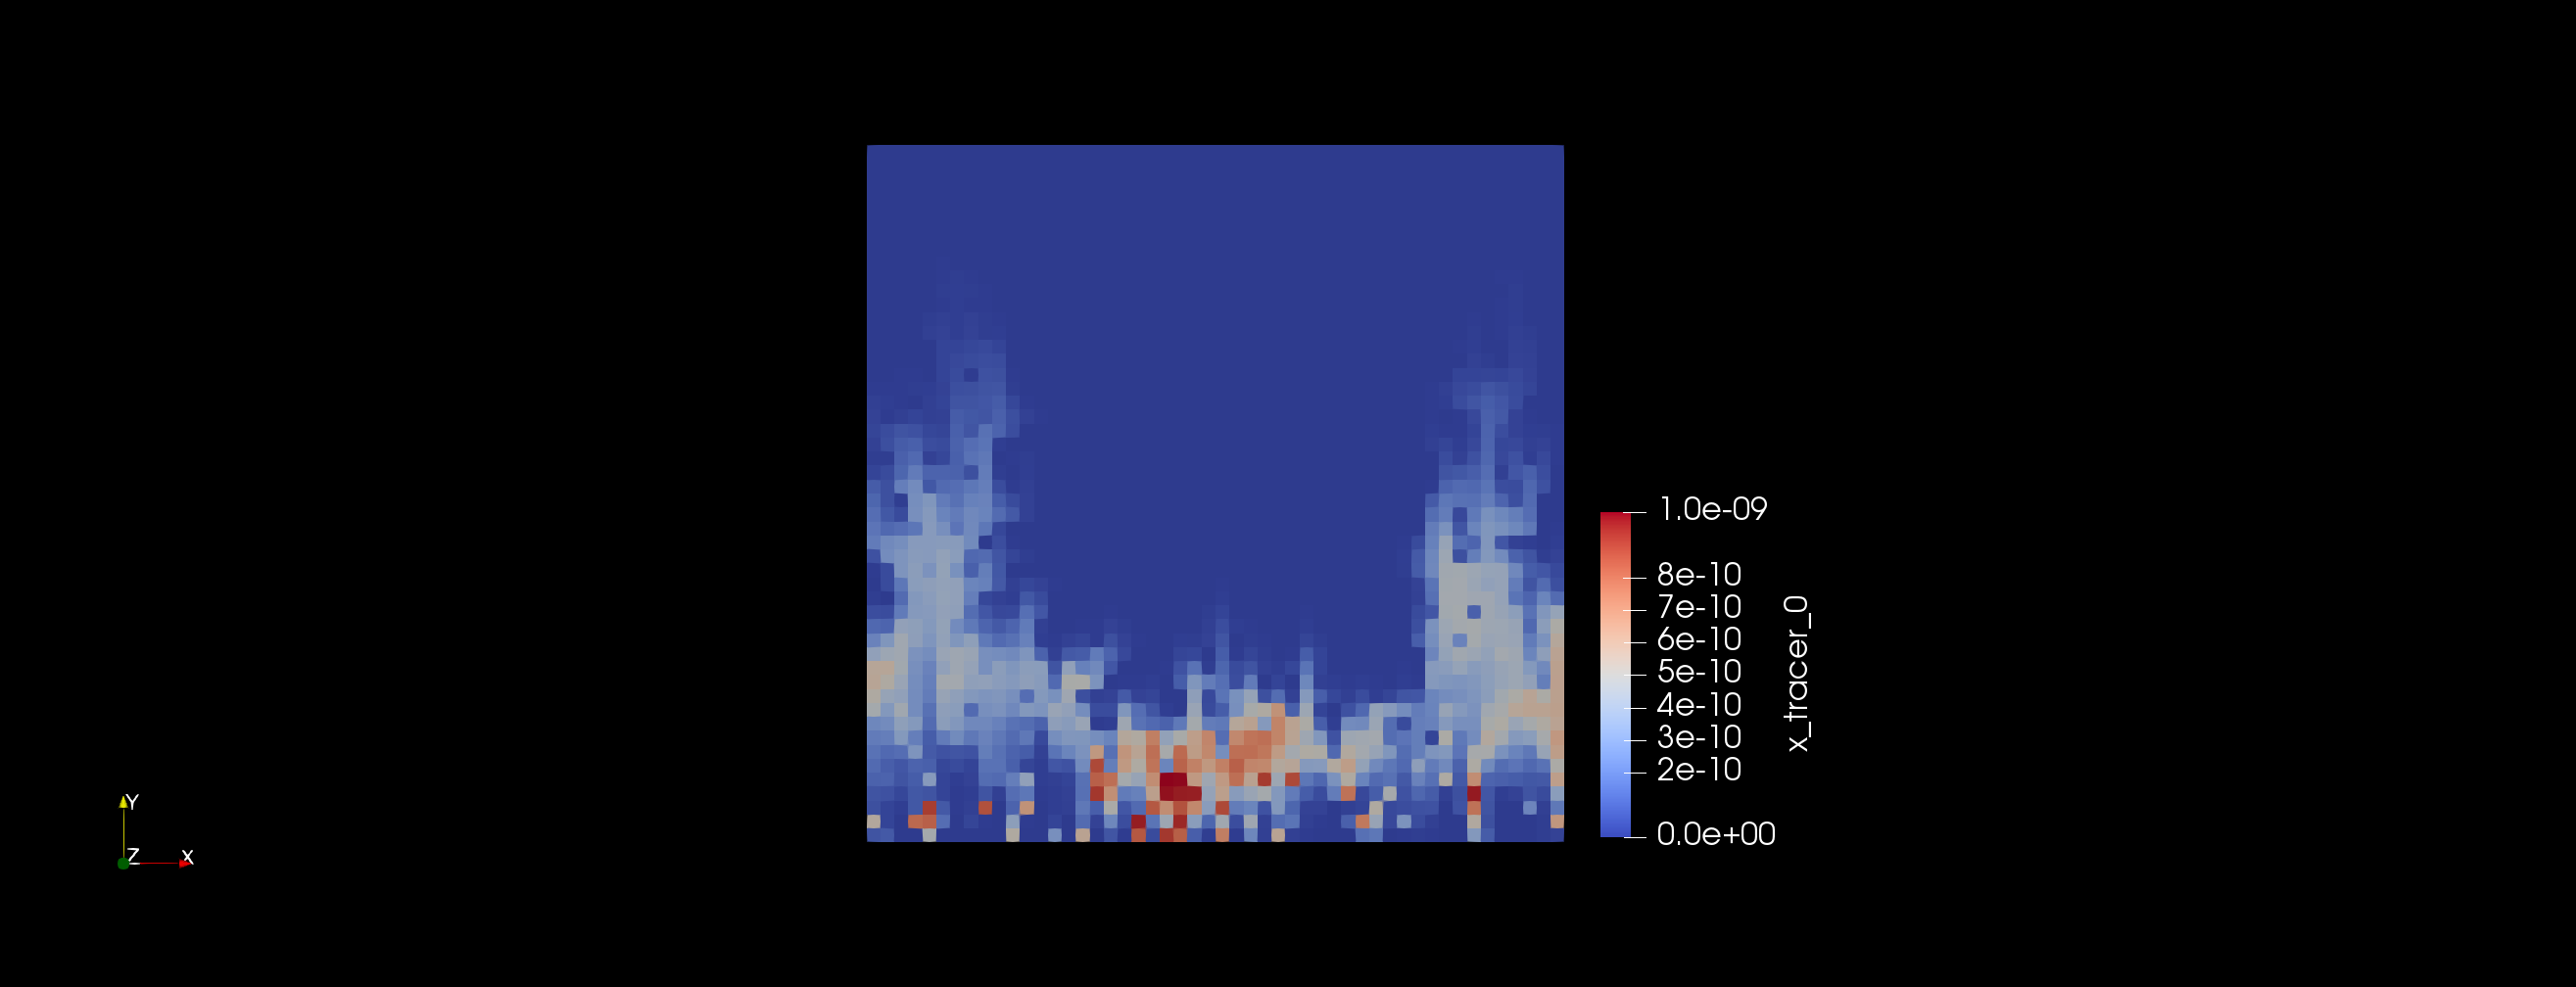
\includegraphics[width=162mm]{tracer_1}
\caption{\footnotesize $DuMu^x$ Tracer Concentration Simulation for a Rectangular Geometry (Time Step 1)}
\label{fig:tracer_1}
\end{figure}
Figure \ref{fig:tracer_1} is the result of a $DuMu^x$ tracer simulation computed on a rectangular geometry. The solute field in the network for the first time step is visualized.\\
\begin{figure}[h]
\centering
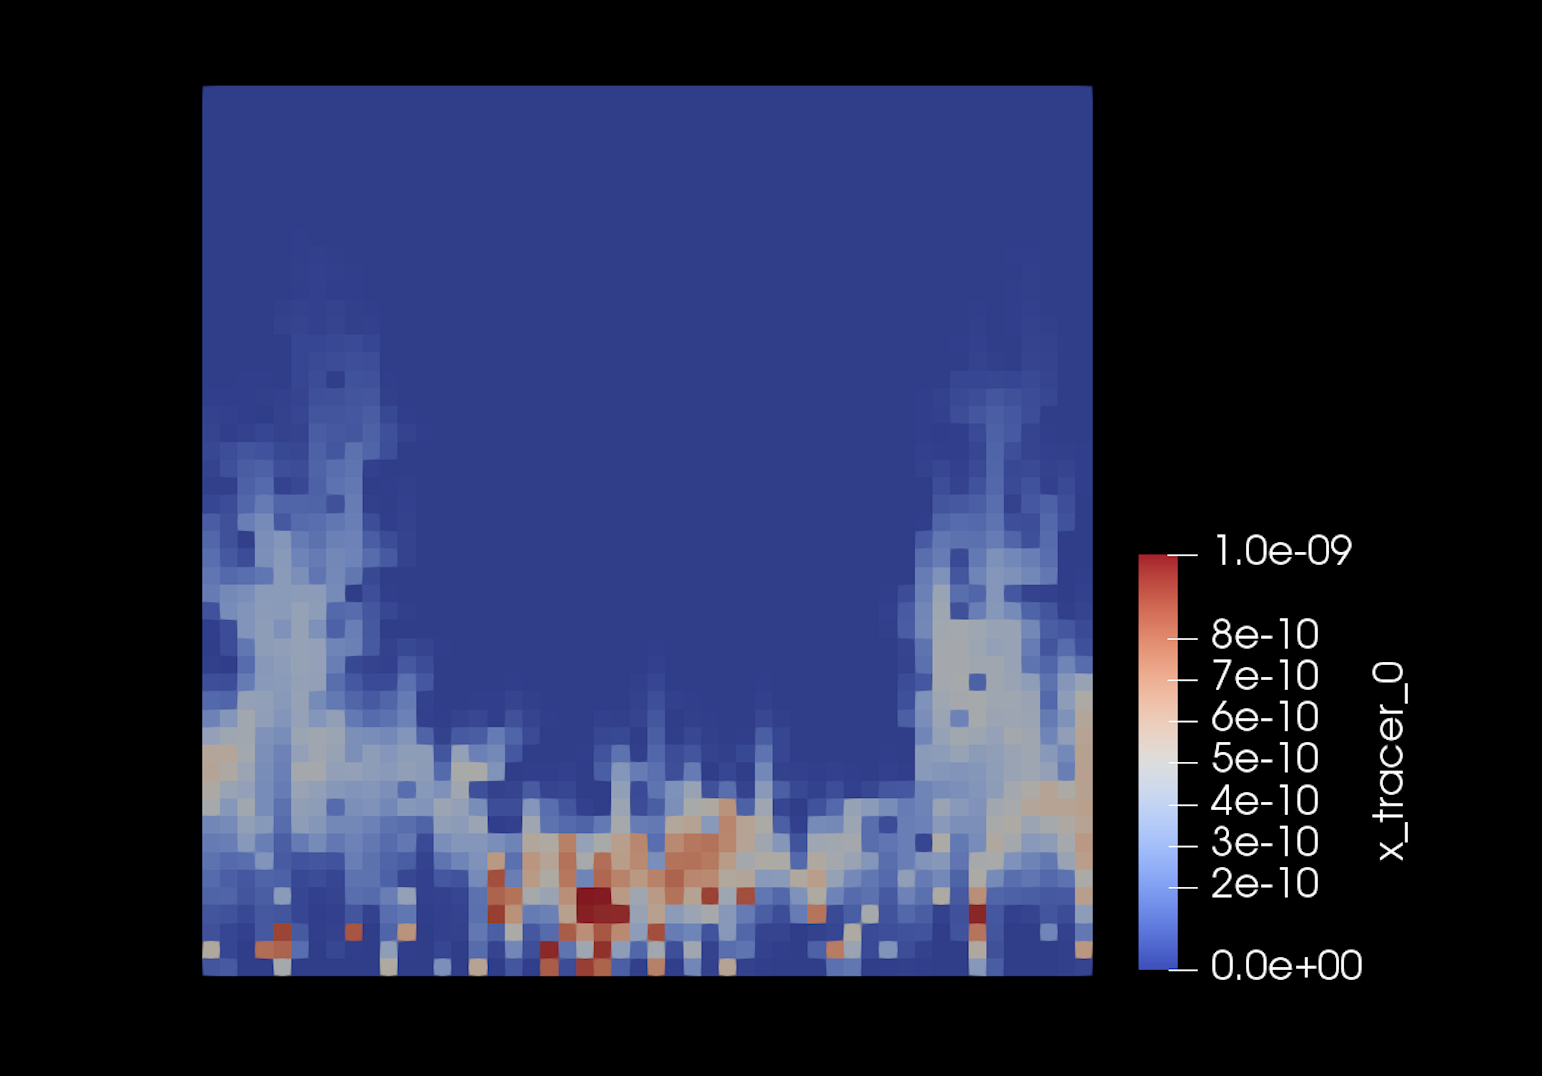
\includegraphics[width=162mm]{tracer_2}
\caption{\footnotesize $DuMu^x$ Tracer Concentration Simulation for a Rectangular Geometry (Time Step 10)}
\label{fig:tracer_2}
\end{figure}
Figure \ref{fig:tracer_2} is the solute field for the same simulation for the last time step is visualized.\\
\begin{figure}[h]
\centering
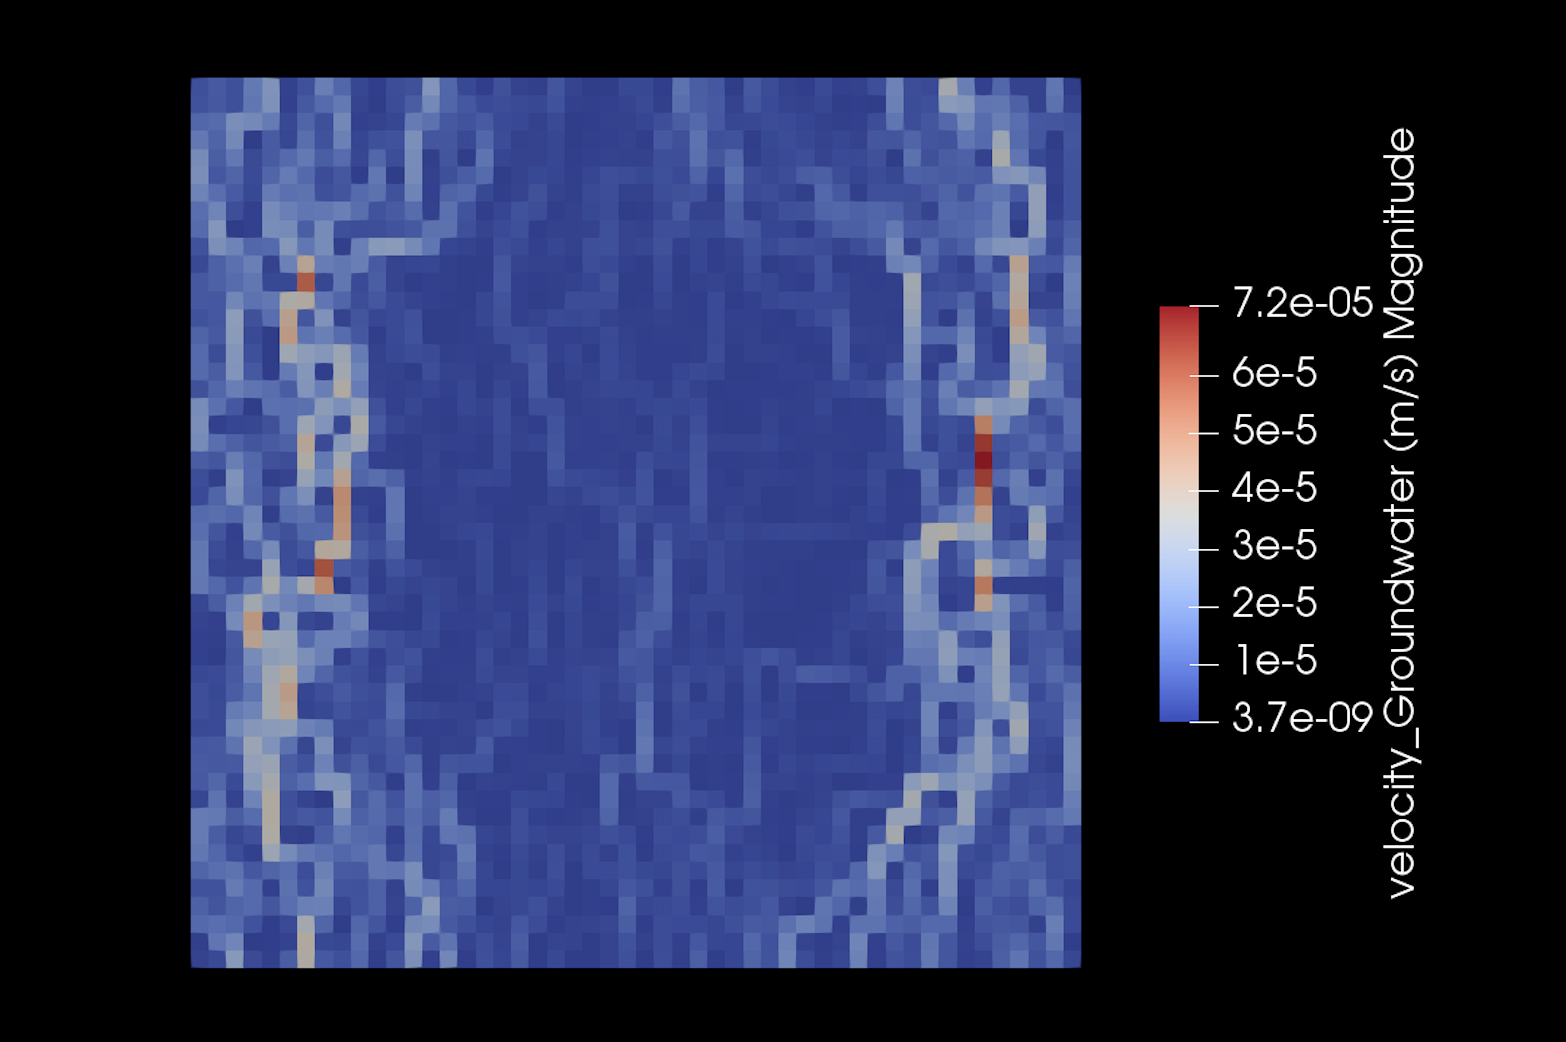
\includegraphics[width=162mm]{tracer_velocity}
\caption{\footnotesize $DuMu^x$ Tracer Velocity Simulation for a Rectangular Geometry}
\label{fig:tracer_velocity}
\end{figure}
Figure \ref{fig:tracer_velocity} is the constant velocity field of the solute.\\